% ══════════════════════════════════════════════════════════════════════════════
\section{High-Bandwidth Memory Regime: Adaptive QR and Large-Scale Simulations}
\label{app:mi355x}
% ══════════════════════════════════════════════════════════════════════════════

Section~\ref{sec:portability} established that \textsc{CppSim} operates in the
memory-bandwidth-bound regime at $\chi \leq 100$ on $4\times4$ grids, where
algorithm choice (Householder vs.\ Cholesky-QR) is invisible in wall-clock time.
This appendix reports what happens when bandwidth is no longer the bottleneck:
a GPU configuration with $5.5\times$ higher memory bandwidth and 192+\,GB VRAM
(GPU-C) shifts the workload into the
compute-bound regime at larger grids, making the Cholesky-QR advantage measurable.
The large VRAM also enables the primary research target --- $10\times10$ at
$\chimax=100$, requiring $\approx109$\,GB.

\subsection{Grid-scaling Trotter timing at $\chi = 50$}

Table~\ref{tab:grid_scaling_mi355x} reports saturated-layer Trotter timing
as ratios relative to each configuration's own $3\times3$ Householder baseline,
so only within-configuration scaling and QR-mode differences are claimed.

\begin{table}[H]
\centering
\caption{Trotter time per layer at $\chi=50$, saturated layers only, normalized
 to the $3\times3$ Householder time within each configuration.
 \texttt{no\_sat}: not all bonds reached $\chi=50$;
 \texttt{---}: run not collected.}
\label{tab:grid_scaling_mi355x}
\smallskip
\small
\begin{tabular}{r r cc cc}
\toprule
& & \multicolumn{2}{c}{GPU-B (ref = $3\times3$ HH)} & \multicolumn{2}{c}{GPU-C (ref = $3\times3$ HH)} \\
\cmidrule(lr){3-4}\cmidrule(lr){5-6}
Grid & Bonds & HH & Adap & HH & Adap \\
\midrule
$3\times3$ & 12 & 1.00 & 1.04 & 1.00 & 0.78 \\
$4\times4$ & 24 & 3.72 & 3.55 & 3.67 & 2.76 \\
$5\times5$ & 40 & 7.57 & 6.86 & 7.62 & 5.55 \\
$6\times6$ & 60 & 12.45 & 11.33 & 12.98 & 8.39 \\
$7\times7$ & 84 & 18.18 & no\_sat & 19.57 & 13.20 \\
$8\times8$ & 112 & no\_sat & no\_sat & 27.71 & --- \\
\bottomrule
\end{tabular}
\end{table}

Both configurations scale identically under Householder QR across all grid
sizes, confirming consistent normalization and the same physical workload.
The \texttt{no\_sat} entries reflect a VRAM ceiling, not a compute or
algorithm limitation.

Cholesky-QR (Adap) tracks Householder within 10\% on GPU-B at all grid sizes,
but progressively pulls ahead on GPU-C --- from 22\% at $3\times3$ to 35\% at
$6\times6$. Sufficient memory bandwidth exposes Cholesky's lower arithmetic
constant; below that threshold, both QR modes are memory-traffic-equivalent.

\begin{figure}[H]
\centering
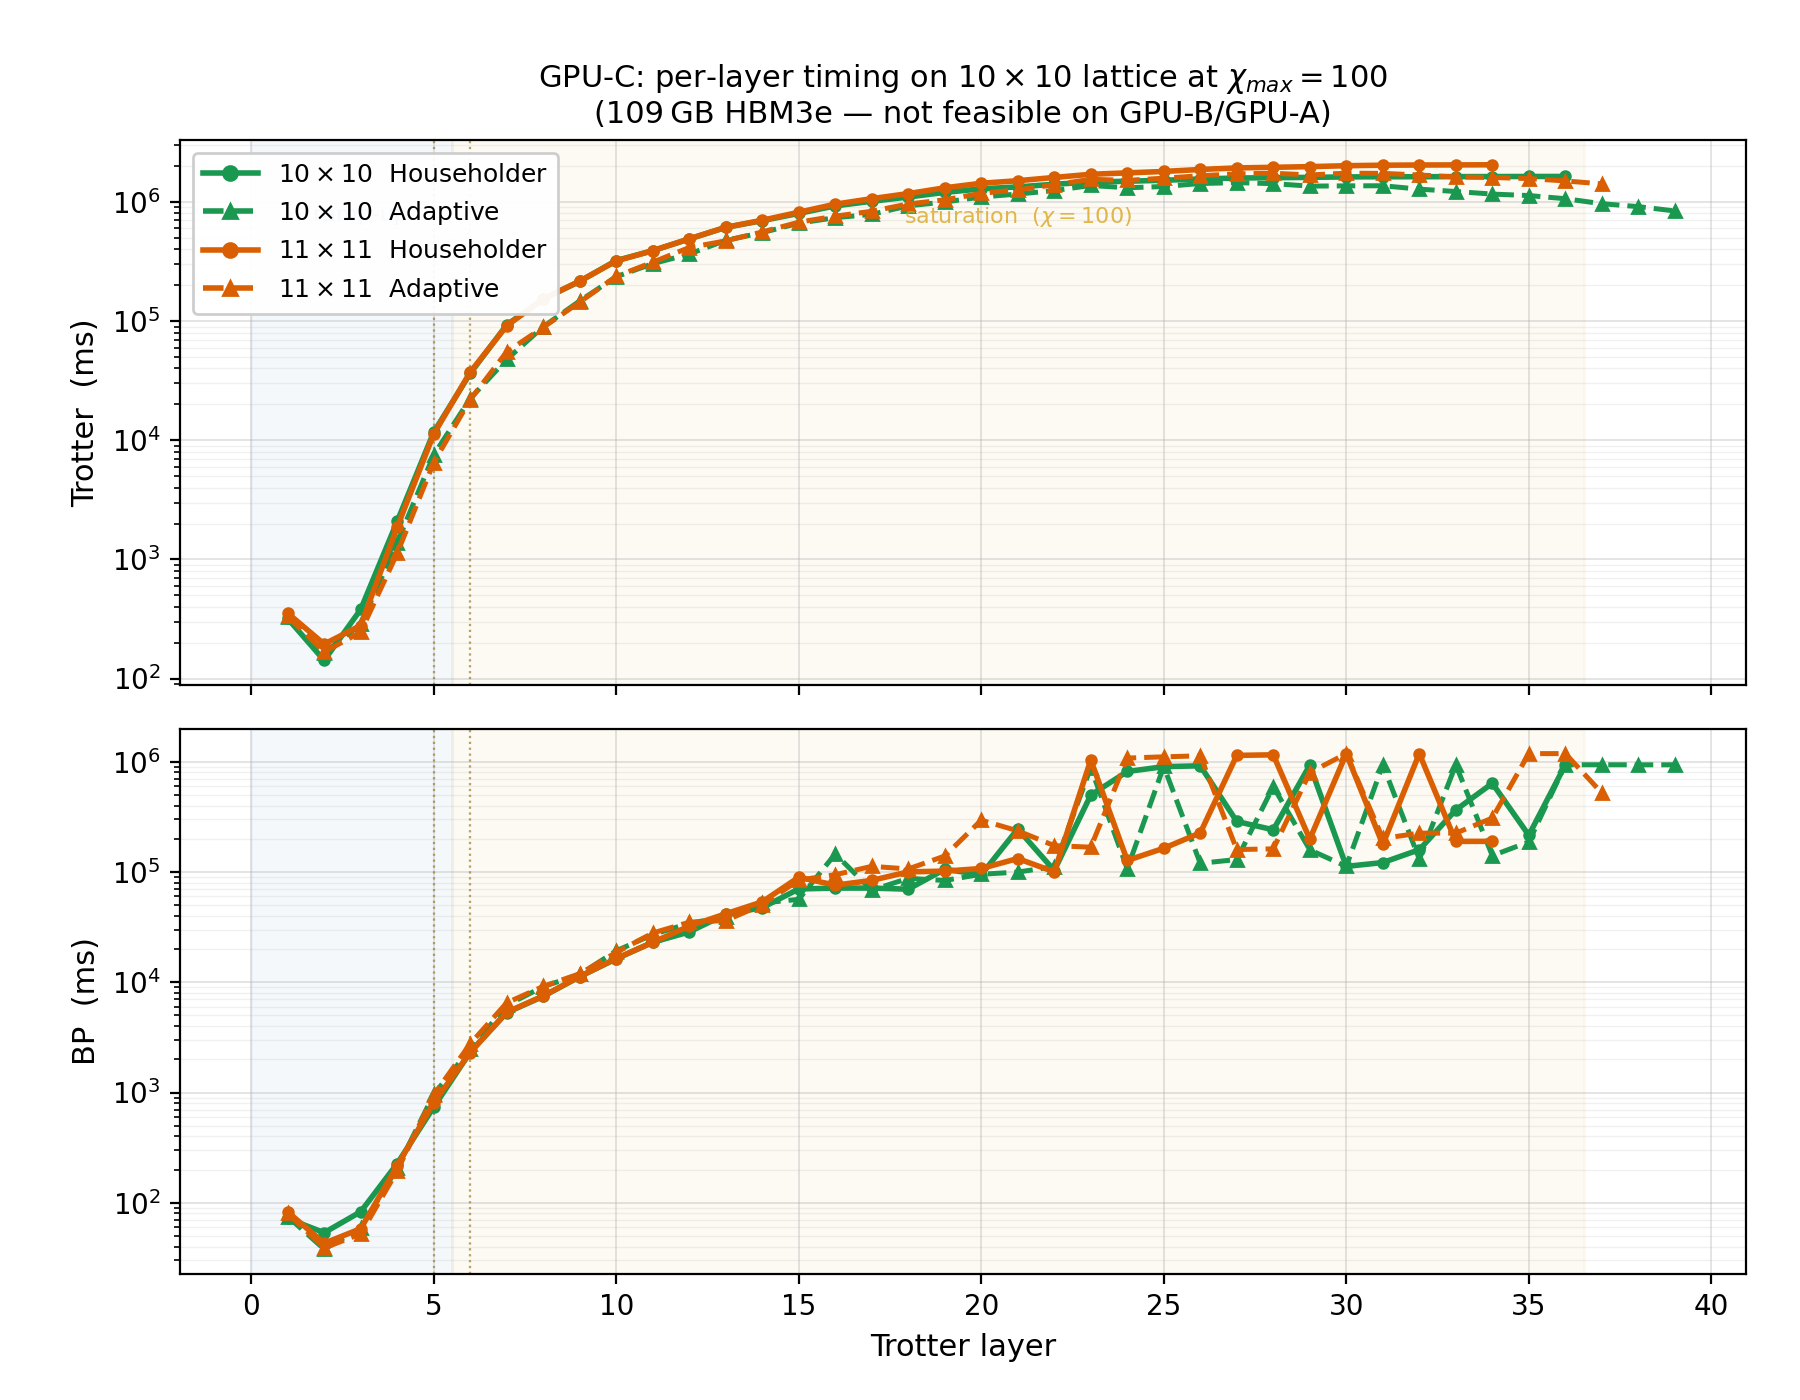
\includegraphics[width=\linewidth]{fig_mi355x_10x10_chi100.png}
\caption{Per-layer Trotter and BP time on the $10\times10$ lattice at
 $\chimax=100$, GPU-C only (high-bandwidth memory, 192+\,GB).
 This run requires $\approx 109$\,GB and is enabled by the 192+\,GB configuration.
 Solid line: Householder QR; dashed: Adaptive QR.
 Trotter time (top) grows smoothly as bond dimension saturates then climbs
 with increasing BP sweep count.
 BP time (bottom) is variable because convergence at $\chi=100$ requires
 up to 100 sweeps (the configured maximum); the spread reflects per-layer
 variation in BP fixed-point difficulty.
 Runs completed 40 of 100 requested layers within the 16\,h wall-time allocation.}
\label{fig:mi355x_10x10_chi100}
\end{figure}

\subsection{BP trap behaviour on GPU-C}

Table~\ref{tab:traps_mi355x} records Type-1 trap occurrences detected by
\texttt{detect\_traps.py} on the GPU-C grid-scaling logs at $\chi=50$.

\begin{table}[H]
\centering
\caption{Type-1 BP traps on GPU-C at $\chi=50$, grid-scaling suite.
 ``none'' = zero Type-1 events in the full run.}
\label{tab:traps_mi355x}
\smallskip
\small
\begin{tabular}{r cc}
\toprule
Grid & HH trap layers & Adap trap layers \\
\midrule
$3\times3$ & 15, 16 & 30 \\
$4\times4$ & 19 & none \\
$5\times5$ & none & none \\
$6\times6$ & none & none \\
$7\times7$ & none & none \\
$8\times8$ & none & --- \\
\bottomrule
\end{tabular}
\end{table}

The pattern is consistent with Table~\ref{tab:trap_inventory}: grids of
$5\times5$ and larger with odd dimensions are trap-free, confirming C4
lattice symmetry as the dominant determinant.
Small grids ($3\times3$, $4\times4$) trap at early layers where all bonds
saturate simultaneously; all Type-1 traps recover within one layer.
Trap layers differ by a few positions across configurations, consistent with
floating-point reduction order selecting a different but equivalent BP path.

\subsection{Spatial operator spreading at $10\times10$}

All $\chi=100$ runs used a 16\,h wall-time allocation, completing ${\approx}38$
Trotter steps (${\approx}70$ for $11\times11$).
These are the first tensor-network simulations of the Heisenberg-picture
Ising model on $10\times10$ and $11\times11$ lattices at $\chi=100$.

At sufficiently long times $C(t)$ decays to zero and the spatial distribution
$n(\mathbf{r},t)$ becomes the primary observable.
We characterize spreading using the per-site non-identity Pauli weight
$n(\mathbf{r},t)$ introduced in \S\ref{sec:lightcone}.
From it we extract two radii --- the mean Manhattan radius $R_{L1}(t)$ and RMS
Euclidean radius $R_{L2}(t)$ from the center site $\mathbf{r}_c$ --- and the
spatial entropy fraction
\begin{equation}
 S_{\rm frac}(t) = \frac{-\sum_{\mathbf{r}} p(\mathbf{r},t)\ln p(\mathbf{r},t)}
 {\ln N^2},
 \quad p(\mathbf{r},t) = \frac{n(\mathbf{r},t)}{\sum_{\mathbf{r}} n(\mathbf{r},t)},
 \label{eq:sfrac}
\end{equation}
the spatial analogue of the bond saturation fraction $S_e/\log\chi$
(\S\ref{sec:experiments}), normalized to $[0,1]$: zero for a perfectly localized
operator, one for uniform weight across all $N^2$ sites.

\begin{figure}[H]
\centering
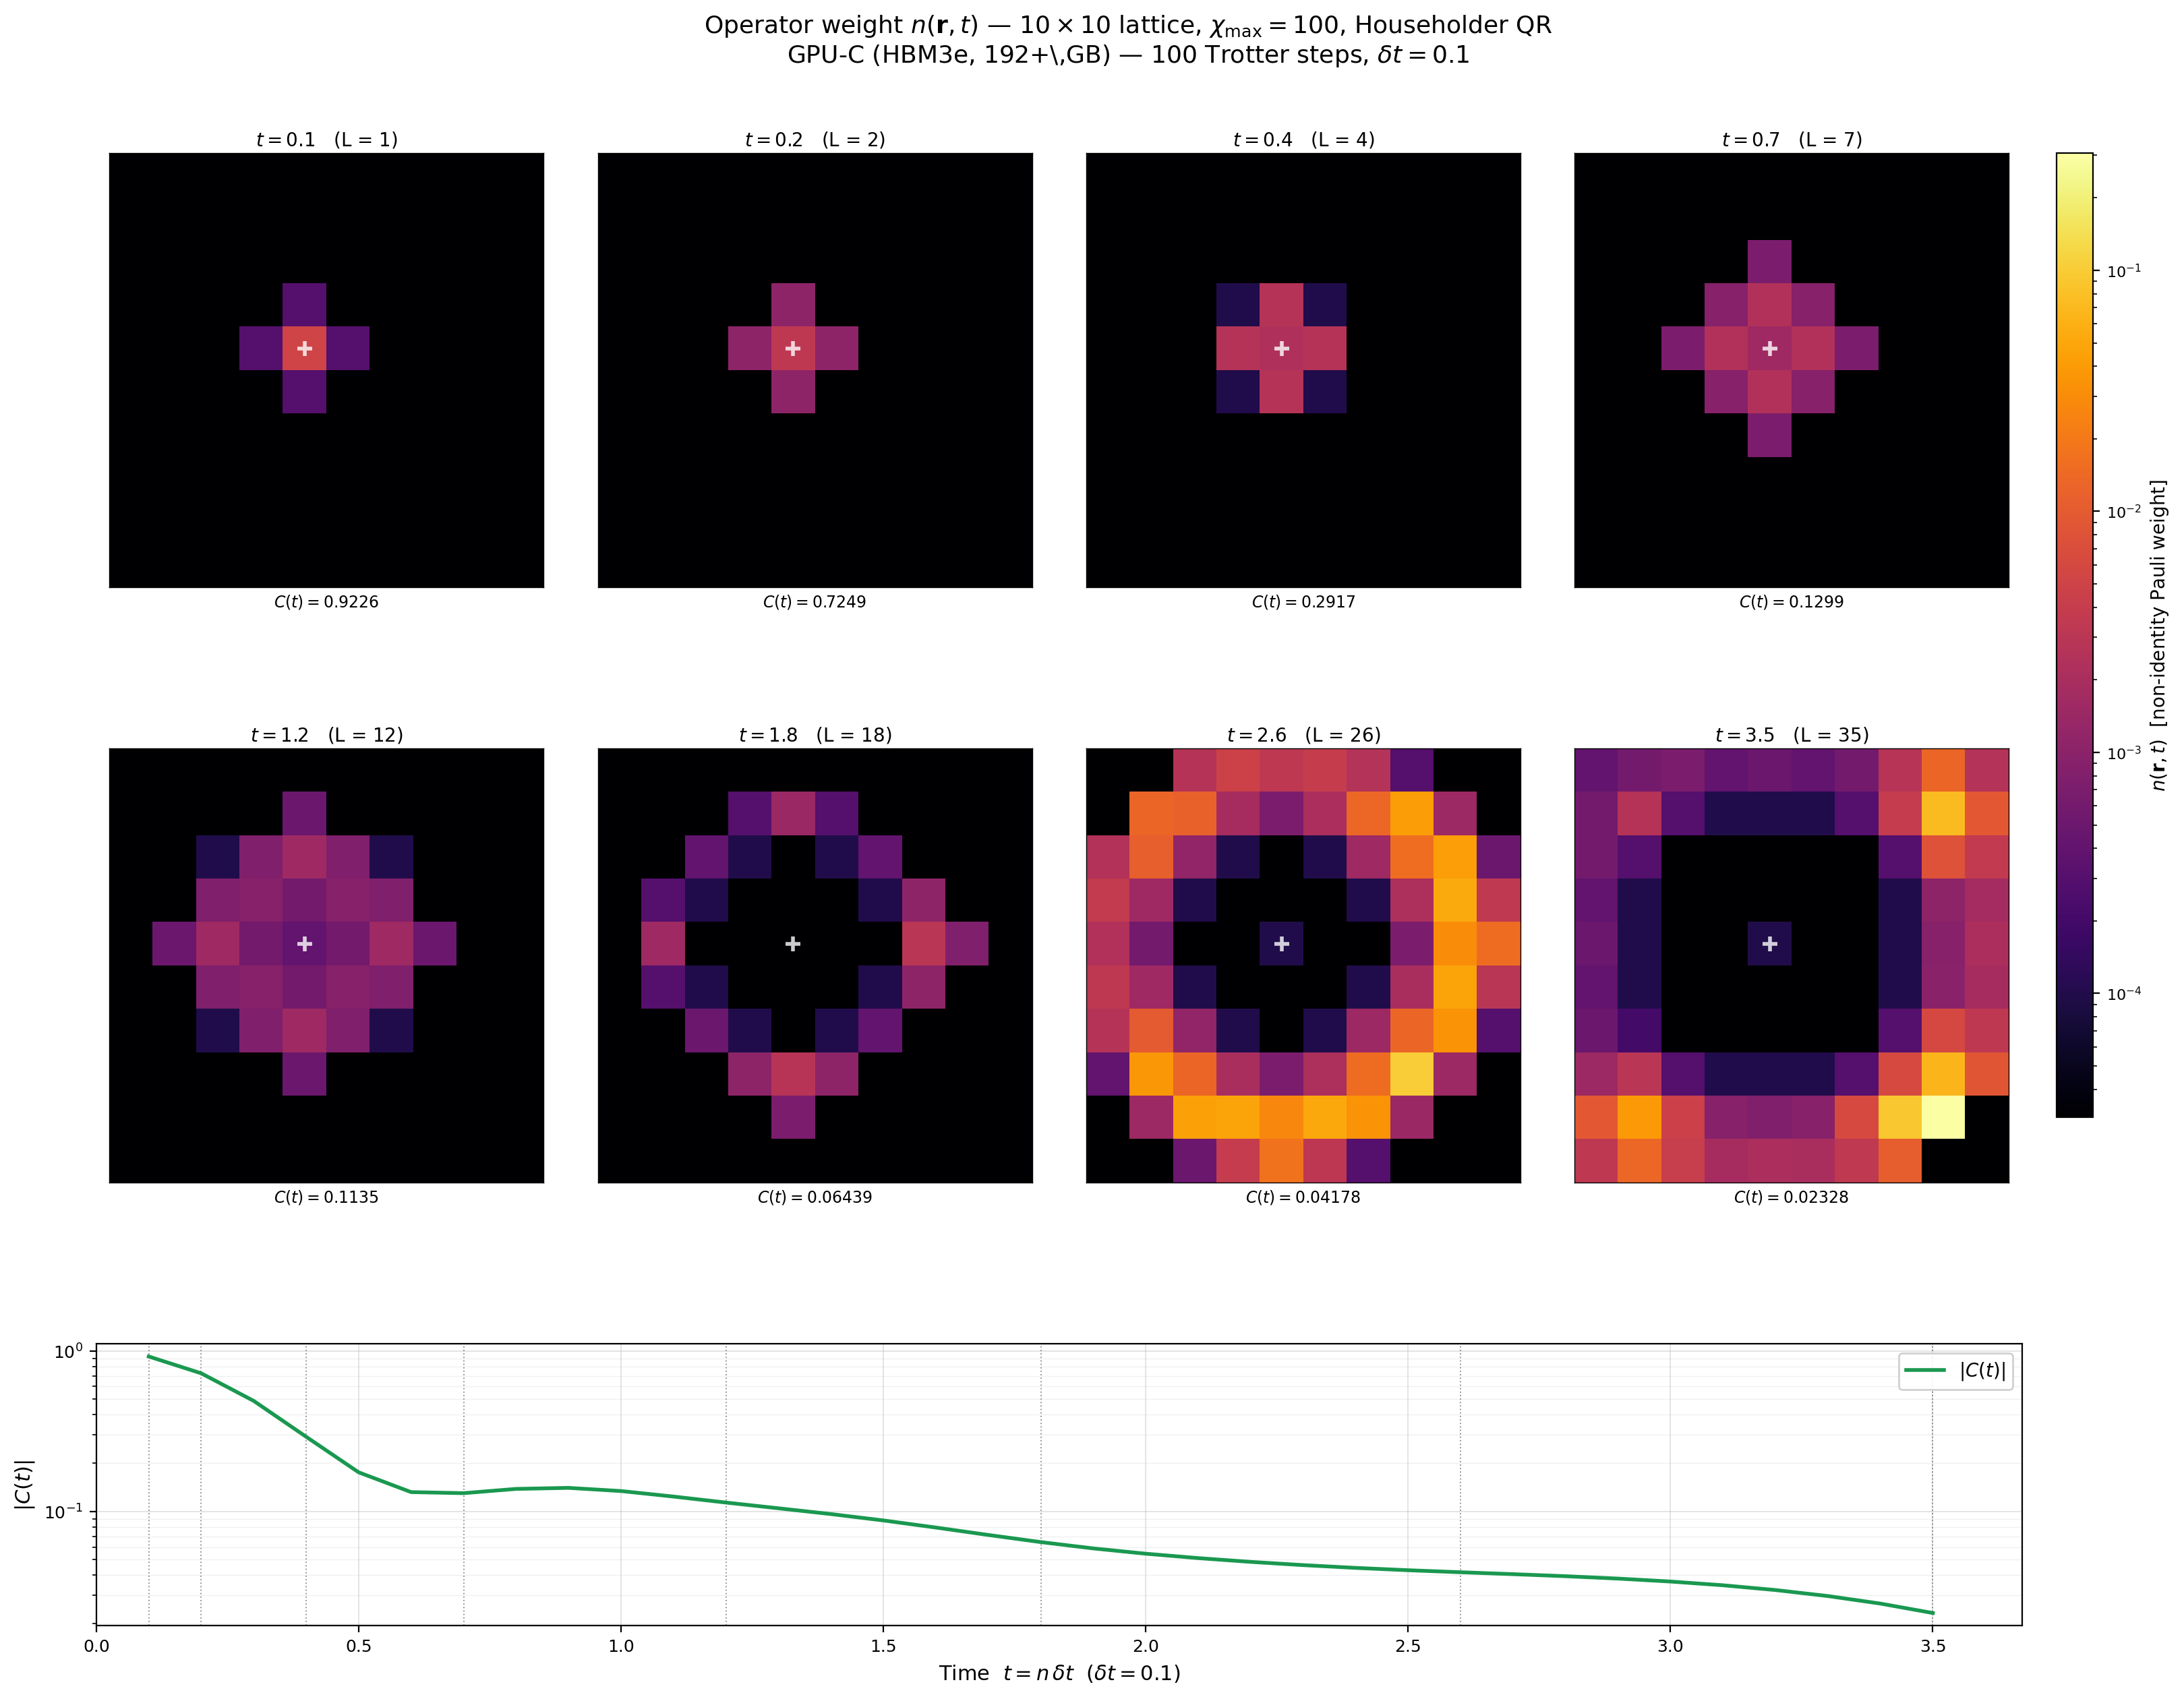
\includegraphics[width=\linewidth]{fig_lightcone_10x10_chi100.png}
\caption{Operator weight $n(\mathbf{r},t)$ on the $10\times10$ lattice at
 $\chimax=100$, Householder QR, eight Trotter snapshots (two rows of four,
 $\delta t = 0.1$).
 The operator starts as a single-site excitation at the center $(4,4)$ and
 expands as a Manhattan-distance diamond (Lieb-Robinson cone).
 At $t \approx 2.0$--$2.4$ the expanding front reaches the lattice boundary
 and reflects, forming a bright ring of accumulated weight at sites equidistant
 from the center.
 At later times the ring disperses toward increasingly uniform coverage
 ($S_{\rm frac} \to 1$).
 \emph{Lower panel}: $C(t)$ decays below $10^{-3}$ by $t \approx 2.0$;
 all physical information at late times is carried by $n(\mathbf{r},t)$,
 not by $C(t)$.
 This run requires $\approx 109$\,GB and is enabled by the 192+\,GB configuration.}
\label{fig:lightcone_10x10}
\end{figure}

\begin{figure}[H]
\centering
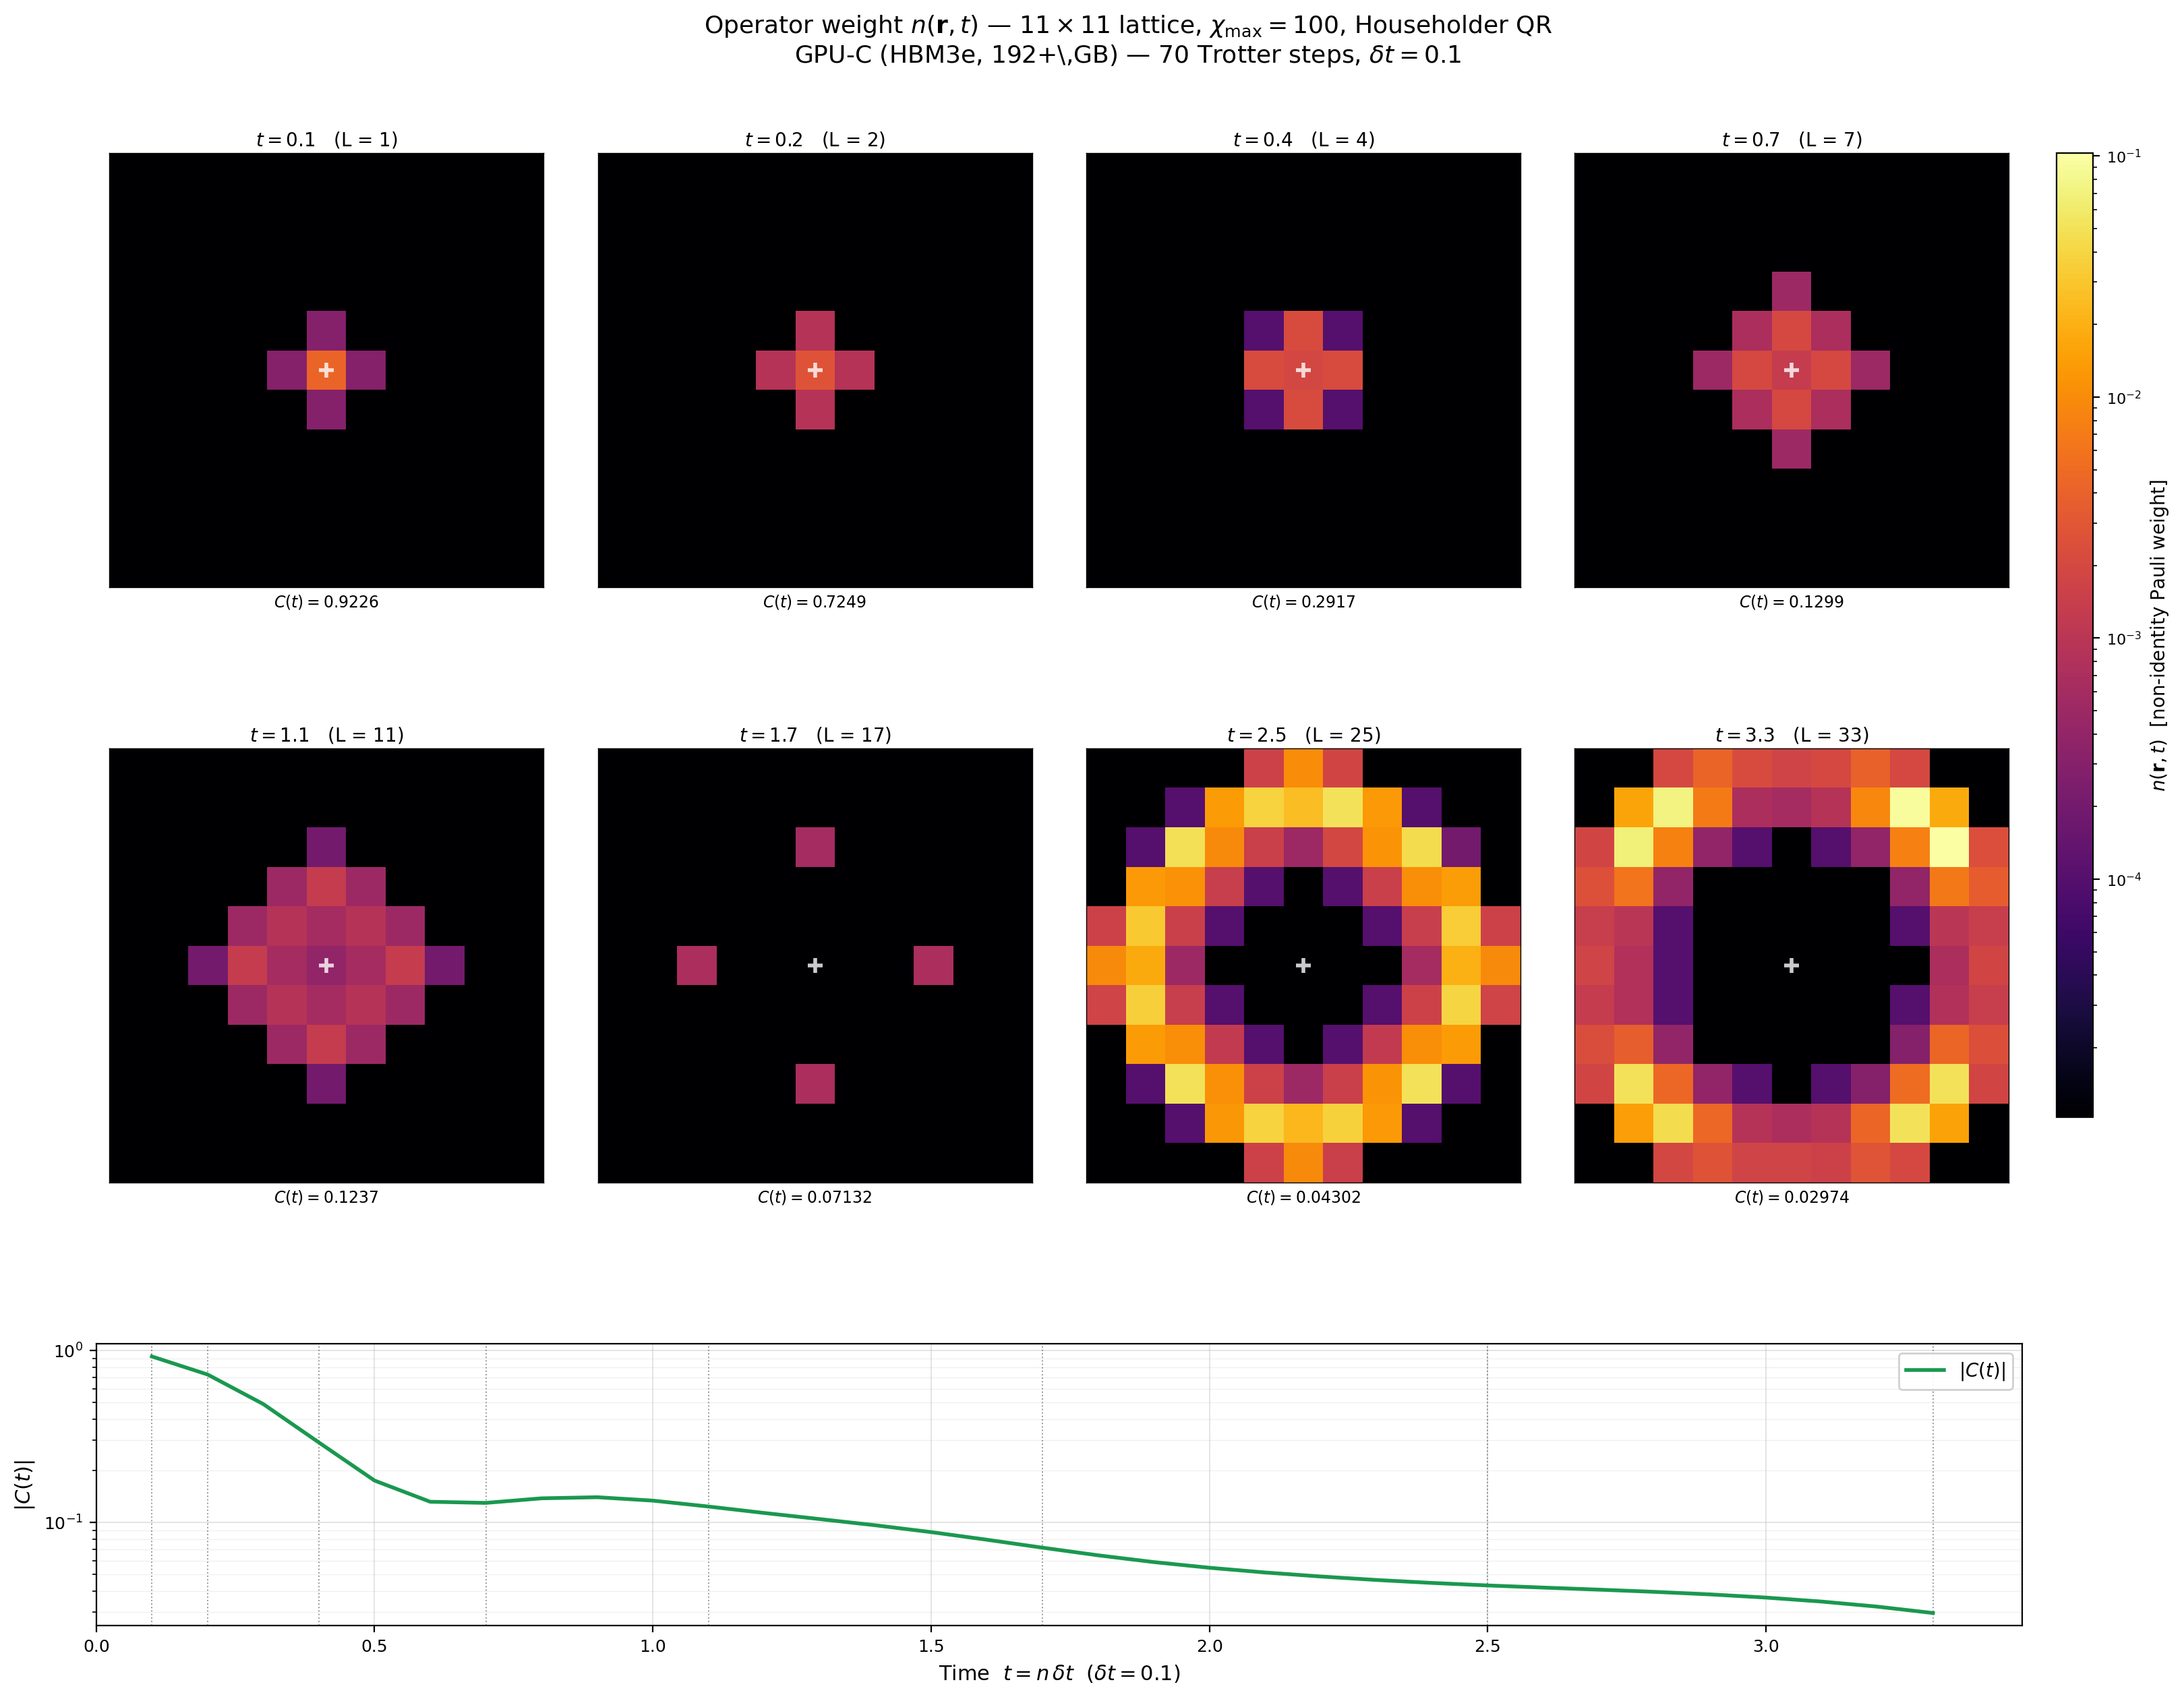
\includegraphics[width=\linewidth]{fig_lightcone_11x11_chi100.png}
\caption{Operator weight $n(\mathbf{r},t)$ on the $11\times11$ lattice at
 $\chimax=100$, Householder QR, eight Trotter snapshots (two rows of four).
 The operator starts as a single-site excitation at the center $(5,5)$.
 \textbf{Early phase} ($t \lesssim 0.7$): ballistic expansion as a
 Manhattan-distance diamond (Lieb-Robinson cone).
 \textbf{Boundary reflection} ($t \approx 1.7$--$2.5$): front reaches all
 four edges; reflected waves form a bright ring equidistant from the center.
 \textbf{Scrambling} ($t \gtrsim 2.5$): ring disperses toward uniform coverage.
 The fourfold C4 symmetry is visible at every layer, confirming zero BP trap
 contamination.
 $C(t)$ (lower panel) decays smoothly to ${\approx}0.03$ over 33 layers.
 This run requires $\approx 130$\,GB and is enabled by the 192+\,GB configuration.}
\label{fig:lightcone_11x11_chi100}
\end{figure}

\subsection{Future performance directions}

Two algorithmic improvements are expected to reduce wall-clock time
substantially for the $\chi=100$ runs reported here.

\paragraph{GPU streams and memory-bandwidth overlap.}
The current implementation applies each Trotter layer synchronously:
the SVD singular values are copied device-to-host to determine the
truncation rank before the next contraction can begin, serialising the
GPU pipeline.
With GPU streams, successive Trotter layers can be overlapped ---
the device-to-host transfer for layer $n$ proceeds concurrently with
the tensor contraction of layer $n+1$.
GPU-C's 192+\,GB high-bandwidth memory capacity is the enabling factor: at $\chi=100$
the full state (${\approx}109$\,GB for $10\times10$, ${\approx}130$\,GB
for $11\times11$) fits comfortably in a single device, leaving sufficient
headroom to double-buffer the workspace tensors required for stream overlap.
On GPU-B (32\,GB) this headroom does not exist; streams are therefore
a GPU-C-specific optimisation.
We estimate a $1.5$--$2\times$ reduction in Trotter time per layer once
the SVD synchronisation point is replaced by an on-device reduction.

\paragraph{Float64 gate arithmetic and Adaptive QR robustness.}
The Adaptive QR mode applies Cholesky-QR as its primary factorisation,
falling back to Householder QR when the Gram matrix is ill-conditioned.
Each fallback incurs a penalty --- visible in the BP timing as a
per-layer spike --- because Householder is slower and resets the gauge
environment for subsequent BP sweeps.
Computing the gate (QR, SVD, Cholesky) in float64 while keeping tensor
storage in float32 would improve Cholesky conditioning significantly:
a well-conditioned Gram matrix produces a more uniform gauge across bonds,
which in turn reduces BP sweep count and eliminates most fallback events.
The space cost is modest (only the gate workspace buffers double, not the
full $O(\chi^2)$ state), and the timing cost is expected to be small
because gate computation is arithmetic-bound in the L2-cache regime
at $\chi \leq 100$.
If fallbacks are eliminated, Adaptive QR would run strictly faster than
Householder at $\chi=100$, making it the unambiguous production mode for
GPU-C across all grid sizes.

